\subsection{CNN Layer Summaries as Feature Vectors}

\todo{better subsection title because it currently sucks}

To understand how semantic concepts of similar granularity are learned by each individual layer in a network we propose a clustering-based approach.  Specifically, for each labeled image on the validation data set, we extract a feature vector that summarizes how each unit is individually activated by the input image, as show in \ref{fig:vectorization}.  The intuition here is that images which activate similar sets of units from the same layer -- and in similar amounts for each unit -- are likely to contain similar visual concepts.  Therefore, this notion of similarity should be captured by the  feature vector, even if the summarization step loses some information (e.g., exact shape location in the image).

Another way to look at this approach is as a collaborative filtering task -- such as in traditional machine learning -- commonly used in recommendation systems.  Whereas a recommendation system would suggest who to follow or what books to buy based on similar ratings in the past, here our collaborative filtering recommends similar images to a candidate image based on similar amounts of activation on the same units in the layer.  If those units activate for similar concepts in a similar fashion, then the final cluster is cohesive and presents visual evidence of that semantic concept. 

\begin{figure}[t]
\centering
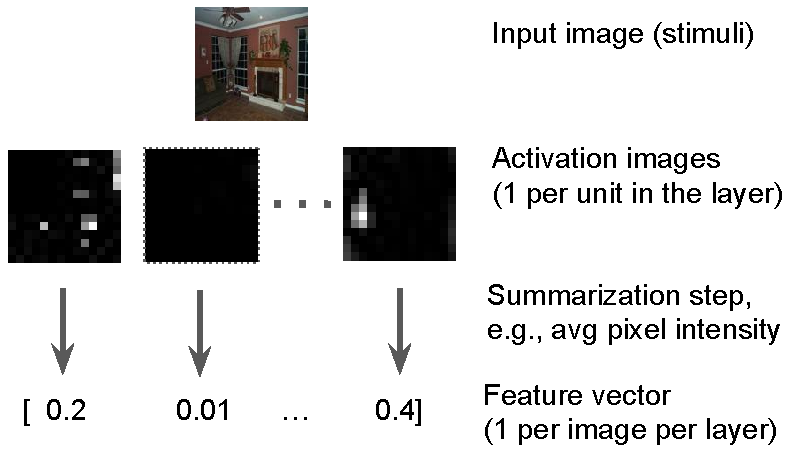
\includegraphics[width=\columnwidth]{figures/vectorization}
\caption{Feature vector obtained for each input image from summarizing its activations on a given CNN layer.}
\label{fig:vectorization}
\end{figure}